%!TEX root = ../thesis.tex
%*******************************************************************************
%****************************** Third Chapter **********************************
%*******************************************************************************
\chapter{pAD}

% **************************** Define Graphics Path **************************
\ifpdf
    \graphicspath{{Chapter3/Figs/Raster/}{Chapter3/Figs/PDF/}{Chapter3/Figs/}}
\else
    \graphicspath{{Chapter3/Figs/Vector/}{Chapter3/Figs/}}
\fi

\section{Phenotype quality control}
With every inpatient visit, patients receive a primary and secondary diagnosis. These diagnoses are recorded using a hierarchical clinical diagnosis framework known as The International Classification of Diseases (ICD) \cite{Hirsch2016-mw}. ICD is a hierarchical framework whereby each medical diagnosis is given an alphanumeric code, and all sub-classifications of any given diagnosis are nested within it. For example, K50 codes for Crohn's disease, while K50.1 codes for Crohn's disease in the large intestine. In this chapter, I will refer to the main ICD codes as "level 1 codes" and their sub-classifications "level 2 codes". The level 1 code for perianal involvement is K60 (K60: Fissure and fistula of the anal and rectal regions)

To understand the genetic architecture of perianal involvement in the general population, I performed a GWAS analysis between all-cause peri-anal disease (pAD) and healthy individuals in the UKBB. 

\subsection{Control exclusion criteria}
To avoid contamination of controls with lower digestive tract disorders that may be true pAD cases that were incorrectly diagnosed, I applied a set of control exclusion criteria. Specifically, I excluded from the control set any individuals who had an ICD-10 hospital diagnosis of K55-K64 and their corresponding ICD-9 codes as demonstrated in Table \ref{table:ukbb_ctrl_excl_criteria}; collectively grouped as "Other diseases of intestines"). These ICD codes indicate symptoms that may resemble pAD symptoms upon presentation, and include ano-rectal bleeding (K55 vascular disorders of the intestine, K57 diverticular disease of intestine and K64 Haemorrhoids and perianal venous thrombosis), or a change in bowel habits (K56 Paralytic ileus and K58 Irritable bowel syndrome), perianal fistula or abscess (K60 fissure and fistula of the anal  and K61), any ano-rectal abnormalities (K62), or proximal fistulas or abscesses (K63). In total, I excluded 133,398 from 481,756 pAD controls (27.7\%).

\subsection{Case inclusion criteria}
To define the case cohort, I identified all individuals with ICD-10 and ICD-9 codes K60
and 565 as case. In total, 5,257 UKBB participants had at least a single visit where they received either a primary or secondary pAD diagnosis or its corresponding ICD-9 code ("anal fissure and fistula"; 565). There are six level 2 codes within K60, representing two broad categories of pAD: fissures and fistulas. Three codes are used for acute and chronic fissures and three codes for acute and chronic fistulas. 92\% of patients (4,858) presented with either K60.1, K60.2 or K60.3 ("chronic anal fissure", "anal fissure, unspecified" and "anal fistula", respectively; Table \ref{table:ukbb_level2_nums}).



\begin{table}[H]
  \centering
  \caption{Number of UKB participant with with a primary or secondary diagnosis for each K60 level 2 code. K60.0=Acute Anal Fissure; K60.1=Chronic Anal Fissure; K60.2=Anal Fissure; unspecified; K60.3=Anal Fistula; K60.4=Rectal Fistula; K60.5= Anorectal Fistula}
  \label{table:ukbb_level2_nums}
  \begin{tabular}{|l|l|l|l|l|l|l|}
  \hline
  ICD-10 code           & K60.0  & K60.1  & K60.2  & K60.3 & K60.4 & K60.5\\ \hline
  Number of individuals & 144                      & 788                        & 2,624                           & 1,954              & 76                   & 122                     \\ \hline
  \end{tabular}
  \end{table}




\begin{table}[]
  \caption{pAD control set exclusion criteria. All ICD-10 codes had corresponding ICD-9 codes except K56 K62 and K63. For those, ICD-9 codes were obtained manually by inspecting level-2 ICD-10 codes and searching for their corresponding level-2 ICD-9 codes.}
  \label{table:ukbb_ctrl_excl_criteria}
  \begin{tabular}{|p{0.1\linewidth}|p{0.2\linewidth}|p{0.2\linewidth}|p{0.3\linewidth}|p{0.1\linewidth}|}
  \hline
  ICD-10 code & ICD-10 meaning                                            & ICD-9 code                          & ICD-9 meaning     & N                                                                                                                                                          \\ \hline
  K55         & Vascular disorders of intestine                           & 557                                 & Vascular insufficiency of intestine       & 2923                                                                                                                                  \\ \hline
  K56         & Paralytic ileus and intestinal obstruction without hernia & 5600, 5601, 5602, 5603, 5608A, 5608, 5609 & Intussusception, Paralytic ileus, Volvulus, Impaction of intestine,Other specified intestinal obstruction, Unspecified intestinal obstruction & 9257                              \\ \hline
  K57         & Diverticular disease of intestine                         & 562                                 & Diverticula of intestine              &     61519                                                                                                                                  \\ \hline
  K58         & Irritable bowel syndrome                                  & 5641                                & Irritable bowel syndrome          & 12418                                                                                                                                          \\ \hline
  K59         & Other functional intestinal disorders                     & 564                                 & Functional digestive disorders not elsewhere classified      & 30087                                                                                                               \\ \hline
  K60         & Fissure and fistula of anal and rectal regions            & 565                                 & Anal fissure and fistula     & 5079                                                                                                                                               \\ \hline
  K61         & Abscess of anal and rectal regions                        & 566                                 & Abscess of anal and rectal regions              &     2178                                                                                                                        \\ \hline
  K62         & Other diseases of anus and rectum                         & 5690, 5691, 5692, 5693, 5694            & Anal and rectal polyp, Rectal prolapse, Stenosis of rectum and anus, Hemorrhage of rectum and anus, Other specified disorders of rectum and anus            & 39191                \\ \hline
  K63         & Other diseases of intestine                               & 5695, 5696, 5697, 5698, 5699            & Abscess of intestine, Colostomy and enterostomy complications, Complications of intestinal pouch, Other specified disorders of intestine, Unspecified disorder of intestine & 33307 \\ \hline
  K64         & Hemorrhoids and perianal venous thrombosis                & 455                                 & Hemorrhoids & 19060\\ \hline

  \end{tabular}
  \end{table}
  \section{pAD cases are enriched in multiple disorders compared to pAD controls}\label{section:pheno_enrich}
  The availability of a large number of clinical diagnoses and phenotypes for UKB participants enables a thorough characterisation of the GWAS case cohort. I aimed to understand the cohort composition and identify which ICD-10 codes are enriched in cases versus controls. For each ICD-10 code, I compared the prevalence in pAD cases versus controls, and I formally tested the enrichment of 1,693 codes using Fisher's exact test. \\

  199 codes were significantly enriched (Fisher’s exact  P-value < $3\times10^{-5}$; Table ). Overall, the enrichment odds ratio was higher than expected (median odds ratio=1.36), likely as a consequence of sampling a disease cohort within a healthy population cohort. 
  
  To understand which groups of disorders were most enriched in pAD cases, I counted the number of enriched disorders within each ICD-10 code categry. I found that five groups had > 10 enriched ICD codes. The largest number of enriched codes belonged to: "Symptoms, signs and abnormal clinical and laboratory findings, not elsewhere classified (R00-R99)" (36 codes), followed by "Diseases of the digestive system (K00-K95)" (34 codes), "Diseases of the genitourinary system (N00-N99)" (22 codes), "Diseases of the musculoskeletal system and connective tissue (M00-M99)" (20 codes), and "Diseases of the skin and subcutaneous tissue (L00-L99)", "Diseases of the circulatory system (I00-I99)" (15 codes).\\
  
  Within digestive systems disorders, ICD-10 code K61 (abscess of anal and rectal regions), followed by K50 (Crohn's disease) were the most significantly enriched (odds ratio=57 and 7.9 respectively). This is expected as a large proportion of pAD patients present with abscess of the perianal region, and perianal fissures and fistulas are known to affect a large proportion of CD patients. Among non-digestive codes, haemorrhoids (I84) was the most significantly enriched diagnosis (P-value=$6\times10^{-98}$; 38\% in pAD cases versus 6\% in controls; odds ratio=9.7). This is likely due to the higher likelihood of diagnosing haemorrhoids in patients with more serious ano-rectal disorders such as pAD, compared to the general population where haemorrhoids patients with no other ano-rectal manifestations are less likely to seek medical advice, and may therefore remain undiagnosed. \\

However, not all enrichments were expected. For example, pAD cases were 1.6 more likely to be diagnosed with gonorthrosis, a gradual erosion of the knee cartialge (P-value=$1.3\times10^-22$; odds ratio=1.6; prevalence in pAD cases is 12\% versus 8\% in controls). A clinical report has previously described chronic arthritis as an "unusual complication" of poorly treated anal fistulas. However, it remains to be answered if such higher prevalence in UKBB can be attributed to poor management or complications, or if it suggests a musculoskeletal or connective tissue pathology underlying fissures and fistulas (a full list of significant enrichments is provided in Appendix A).





  \section{UKBB GWAS}
  Using the pAD case control cohort, I performed a GWAS within UKBB using REGENIE v3.2.5 [ref]. After excluding individuals with missing genotypes or with discordant reported and inferred sex, I conducted the GWAS between 4,606 pAD cases and 332,234 pAD controls (see Methods for genotype data quality control and imputation). After filtering out variants with low imputation quality (INFO < 0.4) and minor allele frequency (MAF) < 0.01, a total of 9,705,089 variants were tested. The GWAS summary statistics exhibited moderate genomic inflation (median $\chi^{2}=0.48$; $\lambda_{GC}=1.06$). Although $\lambda_{GC}$ values up to 1.05 are considered acceptable, higher values can be expected in GWAS with large sample sizes \cite{Price2010-zb}. 
  
  \subsection{Identifying genome-wide significant loci}
  Defining genome-wide significant loci in GWAS studies is often complicated by the widespread correlation between neighbouring genome-wide significant genetic variants (i.e. LD). To identify pAD-associated loci, I used an LD clumping procedure, which outputs a set of \textit{index variants}, each representing a set of highly correlated variants in a locus. Additionally, LD clumping identifies nominally-associated variants that are highly correlated with the index variant at each locus (which I will refer to as LD friends; $R^{2}$ > 0.5 and P-value < 0.01; Methods). In total, seven independent loci achieved genome-wide significant association (P-value < $5\times10^{-8}$). All index variants were well-imputed (INFO $\geq$ 0.99). I also compared the index variants MAFs to population MAFs to ensure that they did not significantly deviate from expected MAFs in NFE. All index variants' MAFs matched MAFs obtained from 1000 Genomes Project (1000GP) and gnomAD v3.1.2, two large sequencing based reference cohorts (see Methods for how MAF deviation from the general population was assessed). 

  \begin{table}[htb]
    \centering\begingroup\fontsize{10}{14}\selectfont
    \caption{genome-wide significant variants in the UKBB analysis. Odds ratio and their 95\% confidence intervals are shown. Minor allele frequencies (MAF) in UKBB and 1000GP are shown in the last two columns.}
    \label{table:gws}
    \begin{tabular}[t]{|l|l|l|l|l|l|l|}
      \hline
      Chromosome & Position & Effect Allele & Odds Ratio & P-value & MAF (UKBB) & MAF (1000GP)\\
      \hline
      3 & 52,992,368 & T & 1.13 (1.08 - 1.17) & 1.5e-08 & 0.42 & 0.44\\
      \hline
      6 & 31,044,486 & G & 1.13 (1.08 - 1.18) & 2.2e-08 & 0.37 & 0.37\\
      \hline
      6 & 31,113,288 & C & 1.13 (1.08 - 1.18) & 1.1e-08 & 0.41 & 0.44\\
      \hline
      6 & 31,113,923 & A & 1.12 (1.08 - 1.17) & 3.2e-08 & 0.49 & 0.49\\
      \hline
      6 & 31,148,469 & A & 1.12 (1.08 - 1.17) & 2.6e-08 & 0.44 & 0.45\\
      \hline
      9 & 22,119,196 & T & 0.89 (0.85 - 0.93) & 2.7e-08 & 0.48 & 0.47\\
      \hline
      11 & 10,356,352 & C & 0.88 (0.84 - 0.92) & 7.3e-09 & 0.29 & 0.30\\
      \hline
      \end{tabular}

    \endgroup{}

    \end{table}

    Four of the seven loci were located in the major histocompatibility complex region (MHC; 6p21.33), and one locus in each of 3p21.1, 9p21.3 and 11p15.4. The MHC region is known to be highly polymorphic and exhibits complex and long-range LD patterns, which complicate the definition of independent loci. 
    For example, two of the four MHC loci overlapped significantly, with their two independent index variant located less than 700 bp apart. One of the two index variants (6:31113288\_T\_C) tagged a large number of variants ($R^{2}$ > 0.8) in the locus, while the other tagged no variants (6:31113923\_A\_G). Compared to the four MHC loci, the three non-MHC loci had less complex LD patterns. All three index variants tagged a large number of variants and none of there was no overlapping independent loci. 


    \begin{figure}[H] 
      \centering    
      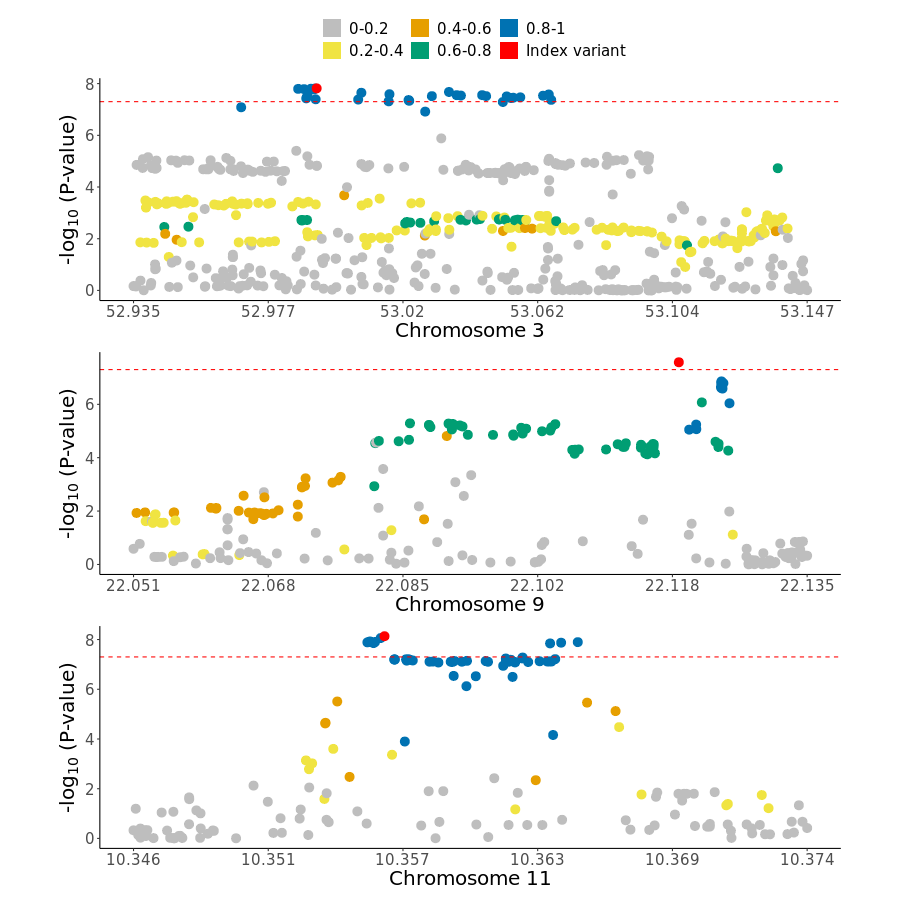
\includegraphics[width=1.0\textwidth]{Vector/ukbb_nonmhc_regional_assoc_plots.png}
      \caption[Figure]{LD decay plots showing association P-values for all four genome-wide significant loci (x-axis) and each variant's $R^{2}$ with the index variant, derived from NFE in 1000GP (y-axis). Red dots and titles indicate the index variant in each locus.}
      \label{fig:ukbb_nonmhc_regional_assoc_plots}
      \end{figure}

      \begin{figure}[H] 
        \centering    
        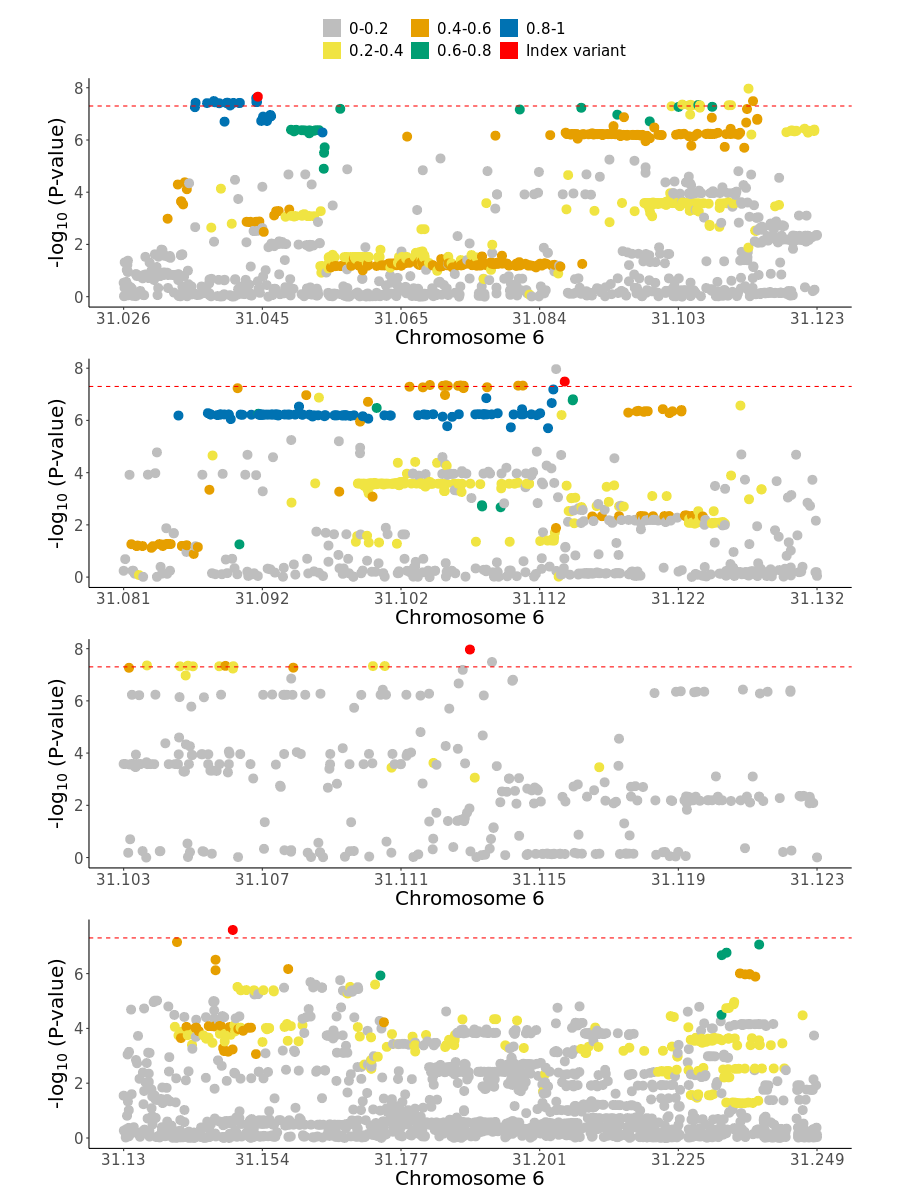
\includegraphics[width=1.0\textwidth]{Vector/ukbb_mhc_regional_assoc_plots.png}
        \caption[Figure]{LD decay plots showing association P-values for all four genome-wide significant loci (x-axis) and each variant's $R^{2}$ with the index variant, derived from NFE in 1000GP (y-axis). Red dots and titles indicate the index variant in each locus.}
        \label{fig:ukbb_mhc_regional_assoc_plots}
        \end{figure}

    \subsection{Post-GWAS quality checks}
    Spurious associations can seriously affect the validity of any significant results in GWAS studies. One of the most common sources of spurious associations is population stratification, which is defined as a systematic difference in allele frequency between subpopulations. At the level of a single locus,  population stratification can be investigated by assessing the relationship between variants' association strength and thir linkage disequllibrium (LD) with the index variant.
    
    I investigated the seven genome-wide significant loci to ensure the association signal follows the expected LD pattern in the general population. For this check to be valid, LD needs to be computed from a suitable matching reference population such as 1000GP. Additionally, each index variant needs to have a number variants in high LD. To this end, I computed LD values with the index variant at each locus from NFE in 1000GP. I assessed the presence of local population stratification by measuring the correlation between $R^{2}$ and P-values of all nominally-associated variants in each of the seven pAD-associated loci.\\

    % \subsection{Index variants quality check}
    
    % All index variants were called in 1000GP except the index variant in 3p21.1 (3:52928665\_C\_T). Despite its high imputation quality in UKBB (INFO=0.93),  3:52928665\_C\_T was flagged as a low-quality site in gnomAD. Gnomad reports that 3:52928665 is a multi-allelic site located in a low-complexity region, and it is covered in fewer than 50\% of gnomAD's individuals. For this locus, I therefore computed LD with respect to the second most significant variant, which was also genome-wide significant (3:52992368\_C\_T; P-value=$1.5\times10^{-8}$). For the remaining three loci, I computed LD with the index variant for all variants in 1mbp window around the index variant. 
    
    \subsection{Relationship between P-value and LD}
  For each of the seven associated loci, I investigated the correlation the $R^{2}$ and P-value of each index variants' LD friends. Index variants in 3p21.1, 9p21.3 and 11p15.4 had LD friends, and the P-values for each index variants' LD friends were highly correlated with $R^{2}$ (Pearson correlation coefficient between $R^{2}$ and $-log_{10}$(P-value) = 0.89, 0.68, 0.72, respectively; Figure), indicating that the P-values closely match the expected LD pattern in
  NFE. Two of the MHC loci also showed a similar pattern (index variants 6:31044486\_G\_C and 6:31148469\_G\_A), with a strong correlation between P-values and $R^{2}$ (Figure). However, this correlation did not hold for the two other overlapping MHC loci.
  
  \subsubsection{A complex LD pattern at two MHC loci}
  \begin{figure}[H] 
    \centering    
    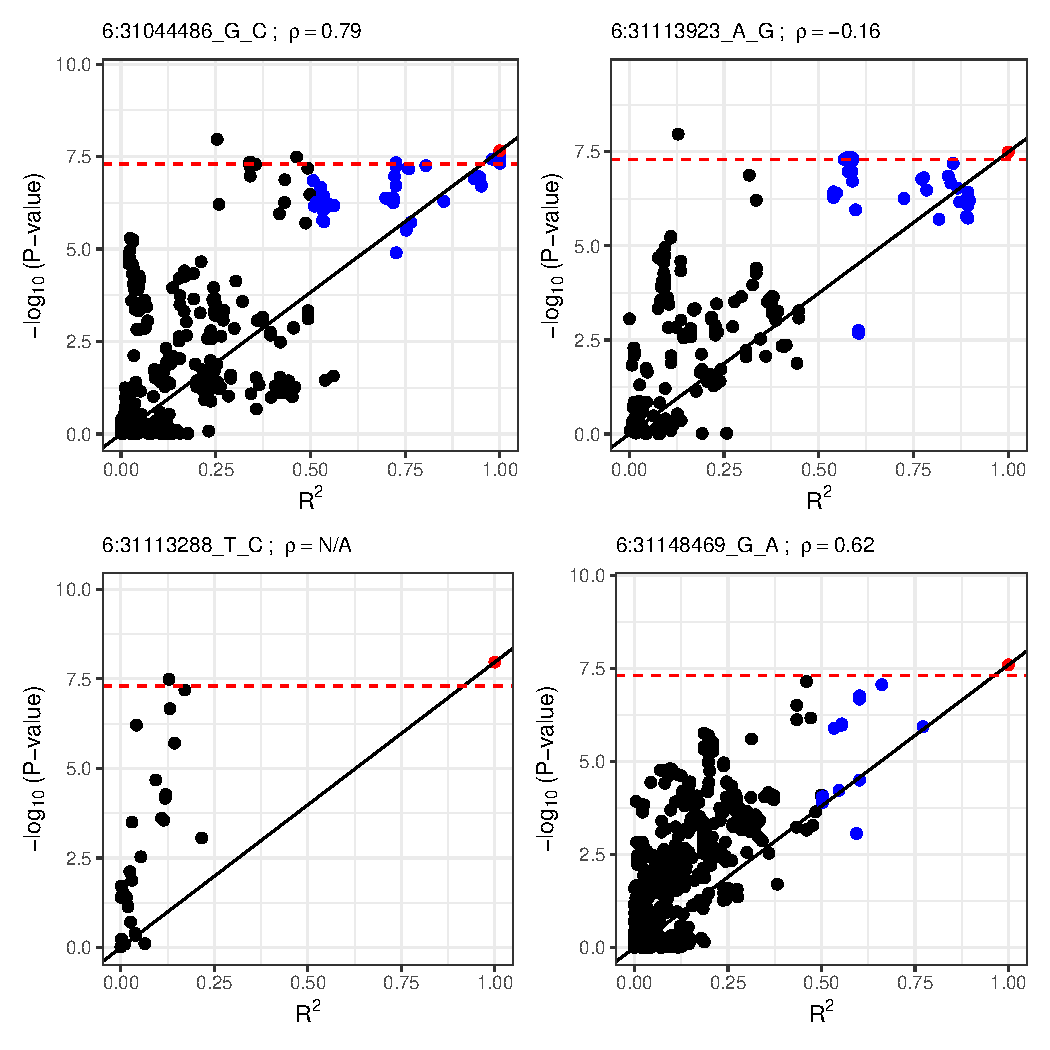
\includegraphics[width=0.8\textwidth]{ukbb_ld_decay_mhc}
    \caption[Figure]{LD decay plots showing association P-values for the four genome-wide significant loci in the MHC locus (x-axis) and each variant's $R^{2}$ with the index variant, derived from NFE in 1000GP (y-axis). Red dots and titles indicate the index variant in each locus. }
    \label{fig:ukbb_ld_decay_mhc}
    \end{figure}
  First, one of MHC index variants at the two overlapping MHC loci did not tag any LD friends and therefore the correlation between P-value and $R^{2}$ could not be assessed (6:31113288\_T\_C; Figure). It is unclear whether the absence of LD friends for 6:31113288\_T\_C suggests that it is a truly indepent variant, or whether it is driven by a mismatch between the LD patterns in UKBB and 1000GP. Such a mismatch may lead to an underestimateion of LD between the index variant and its LD friends. To answer this question, I recalculated the LD values in 1000GP using only British individuals (GBR; N=90), and found that the index variant also did not tag any LD friends in GBR. Given that 6:31113288\_T\_C is well-imputed (INFO=0.99) and common and that it is not well-tagged in both the NFE and GBR subpopulation in 1000GP, it is unlikely that the its association is driven by local population stratification.

  \begin{figure}[H] 
    \centering    
    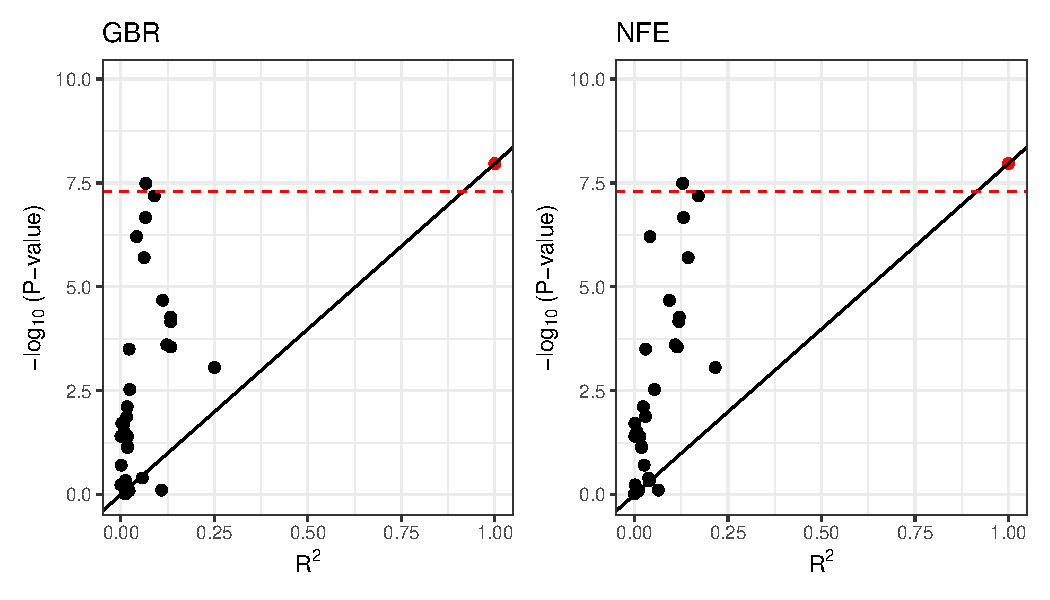
\includegraphics[width=0.8\textwidth]{ukbb_ld_decay_nfe_vs_gbr}
    \caption[Figure]{LD decay plots showing association P-values for 6p21.33 and each variant's $R^{2}$ with the index variant, derived from NFE and GBR in 1000GP (y-axis), showing that the index variant does not have any LD friends in both NFE and GBR. Red dots and titles indicate the index variant.}
    \label{fig:ukbb_ld_decay_nfe_vs_gbr}
    \end{figure}

  Second, for the second overlapping locus, $R^{2}$ and P-values showed an opposite correlation (Pearson correlation coefficient between $R^{2}$ and $-log_{10}$(P-value)=-0.16). Such an unexpected inverse correlation between $R^{2}$ and P-values suggest that not all the LD friends' P-values conform to their expected P-values given their LD with the index variant. I hypothesised that the reversal of correlation may be caused by the subset of LD friends with $R^{2}$ close to the value used for defining LD friends. This subset could lead to a reversed correlation due to a lower-than-expected P-value given their LD with the index variant. To this effect, I found that 10 LD friends had a genome-wide significant P-value (< $5\times10^{-8}$) despite all having an $R^{2}$ of 0.58 with the index variant. When I repeated the LD clumping procedure at this locus with a higher clumping $R^{2}$ cutoff (=0.6), I found that this subset of variants constituted a new genome-wide significant locus. This suggests that the identification of independent loci at this region is senstitive to the choice of LD clumping $R^{2}$ cutoff. 
  

  



      \section{Finngen GWAS}
      Similar to UKBB, other national biobanks with genetic, clinical and phenotypic are available. Although most national biobanks limit access to their individual-level genotype and phenotype data to approved researchers only, results from secondary analyses, including GWAS summary statistics, are made publicly available. \\

      Finngen is a national biobank whose aim is to collect genetic and phenotypic data for 500,000 Finnish individuals. The latest data freeze (Data Freeze 9) has genotyped over 377,000 individuals and provides over 2,200 clinical endpoints. Although I do not have access to individual-level data, GWAS summary stiatistics for all Finngen phenotypes are made pubicly available, and can even be browsed interactively (r9.finngen.fi/).\\

  Finngen uses a different clinical coding system from ICD to organise phenotypes into endpoints (Finngen endpoints). There are two main differences between UKBB and Finngen in terms of their clinical code structure. First, most Finngen endpoints have parallel ICD codes, but additional Finngen endpoints are created at request. Bespoke endpoints define certain inclusion or exclusion criteria based on ICD codes, or sometimes combine codes from different ICD chapters to create a new endpoint. Second, Finngen endpoints are curated by experts in each field and are constantly reviewed in different Finngen data freezes, and are classified as \textit{core endpoints}, or \textit{non-core endpoints}. Basic statistics such as prevalence and gender ration are calculated for all Finngen endpoints, while GWAS is conducted only for core endpoints.\\

ICD-10 code K60 corresponds to Finngen endpoint K11\_FISSANAL. K11\_FISSANAL defineds cases and controls similar to my UKBB cohort definition outlined in Table \ref{table:ukbb_ctrl_excl_criteria}. K11\_FISSANAL was considered a core endpoint until Data Freeze 7, and GWAS summary statistics for K11\_FISSANAL are threfore unavailable in later data freezes. 

\subsection{Identification of genome-wide significant loci in Finngen}

In order to investigate if the seven UKBB genome-wide significant loci replicated in an independent cohort and to identify additional loci, I downloaded GWAS summary statistics for Finngen's clinical endpoint K11\_FISSANAL. As of data freeze 7, Finngen reports 6,610 pAD cases and 253,186 controls. There was no information regarding the subtypes of pAD (e.g. fissures and controls), and it is therefore unclear if the composition of Finngen's pAD case cohort is similar to the UKBB pAD case cohort. Understanding the differences in subphenotype composition of each cohort between the UKBB and Finngen is important to understand if differences in association at genome-wide significant loci is driven by genetic factors (e.g. differences in MAFs) or by phenotypic differences between the cohorts. 

After I filtered out variants with MAF < 0.01, a total of 9,054,355 variants remained. There was an acceptable level of genomic inflation (median $\chi^{2}$=0.495; $\lambda_{GC}$=1.089). To identify genome-wide significant loci, I used an LD clumping approach similar to the UKBB analysis, with the only difference being that I calculated LD from Finnish Europeans in 1000GP (FE; N=99). I found three genome-wide significant non-MHC loci: 1p34.2, 6p25.3 and 12q24.21 (P-value < $5\times10^{-8}$). Imputation quality information was not available in the downloaded summary statistics, so I was not able to confirm if the index variants had good imputation quality. However, the index variants' MAFs matched MAFs derived from FE in 1000GP, suggesting that they are imputed or genotyped with high confidence. Furthermore, I performed similar post-GWAS checks to UKBB to ensure the P-value of the index variants LD friends match their expected values given their LD with the index variant. At the three loci, all LD friends P-values showed the expected correlation with their LD value with the index variant ($\rho$=0.92, 0.74 and 0.44, respectively)

\begin{table}[htb]
  \centering\begingroup\fontsize{10}{12}\selectfont
  \caption{}
  \label{table:gws_finngen}
  \begin{tabular}[t]{|l|l|l|l|l|l|l|}
  \hline
  Chromosome & Position & Effect Allele & Odds Ratio & P-value & MAF (Finngen) & MAF (1000GP)\\
  \hline
  1 & 39,817,036 & T & 1.14 (1.09 - 1.19) & 7.2e-10 & 0.21 & 0.22\\
  \hline
  6 & 1,771,278 & T & 0.9 (0.87 - 0.93) & 6.7e-09 & 0.42 & 0.39\\
  \hline
  12 & 114,235,969 & T & 1.11 (1.07 - 1.15) & 7.0e-09 & 0.47 & 0.47\\
  \hline
  \end{tabular}
  \endgroup{}
  \end{table}

\begin{figure}[H] 
  \centering    
  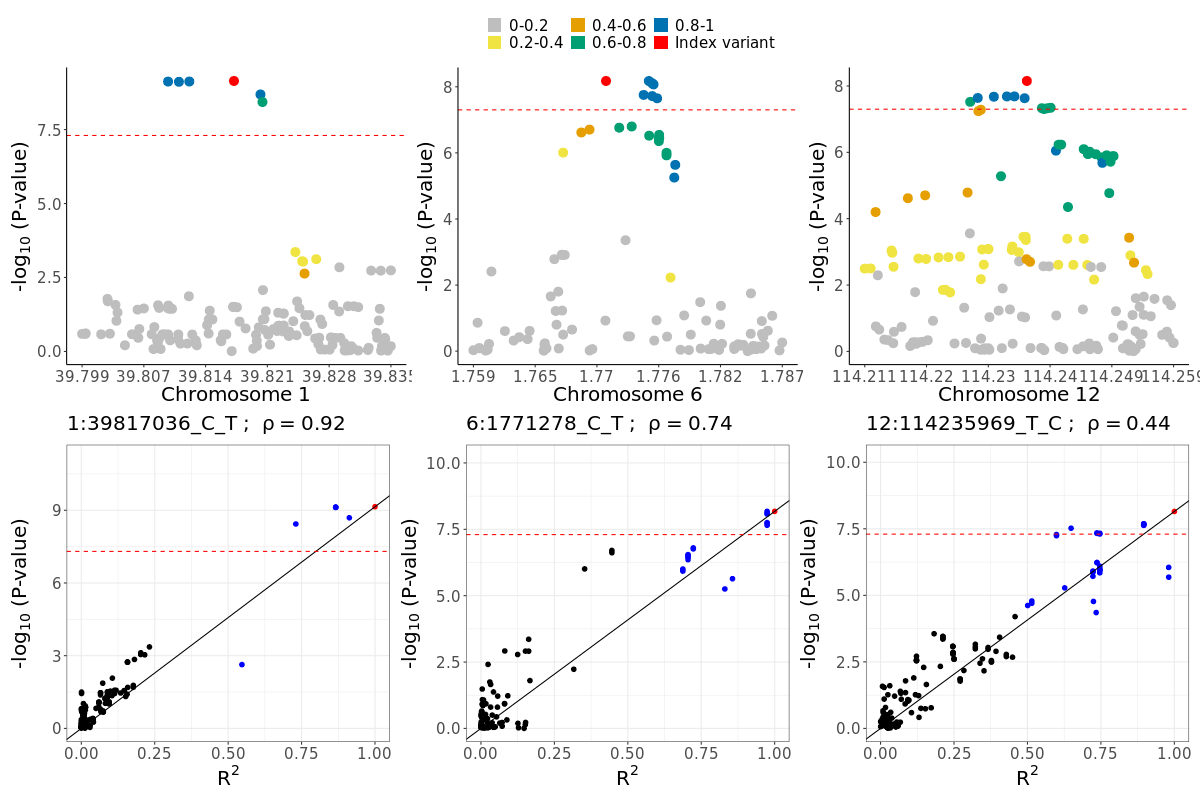
\includegraphics[width=1.0\textwidth]{Vector/finngen_regional_assoc_ld_decay_plots.png}
  \caption[Figure]{}
  \label{fig:finngen_regional_assoc_ld_decay_plots}
  \end{figure}




\subsection{Replication of UKBB loci in Finngen}

\subsubsection{LD pattern in Finnish Europeans}
In GWAS studies, the true causal variant in an associated locus is often unknown due to LD between variants. Moreover, it is often the case that the true causal variant may not even be genotyped in array-based GWAS studies. When assessing replication of a GWAS locus between two cohorts, it is therefore important that their LD structure is similar. Indeed, a lack of GWAS hit replication is sometimes driven by a difference in LD patterns between the two subpopulations under comparison, one of which may not have genotyped or imputed any variants that tag the true causal variant \cite{Kraft2009-xg}. Finnish Europeans (FE) and NFE are known to exhibit systematic difference in their LD strucure, which may affect the ability to replicate the pAD-associated loci discovered in the UKBB. To compare the LD pattern between FE and NFE at the pAD-associated loci, I computed the LD between each variant and the index variant in the FE and NFE subpopulations of 1000GP.\\





% \begin{figure}[H] 
%   \centering    
%   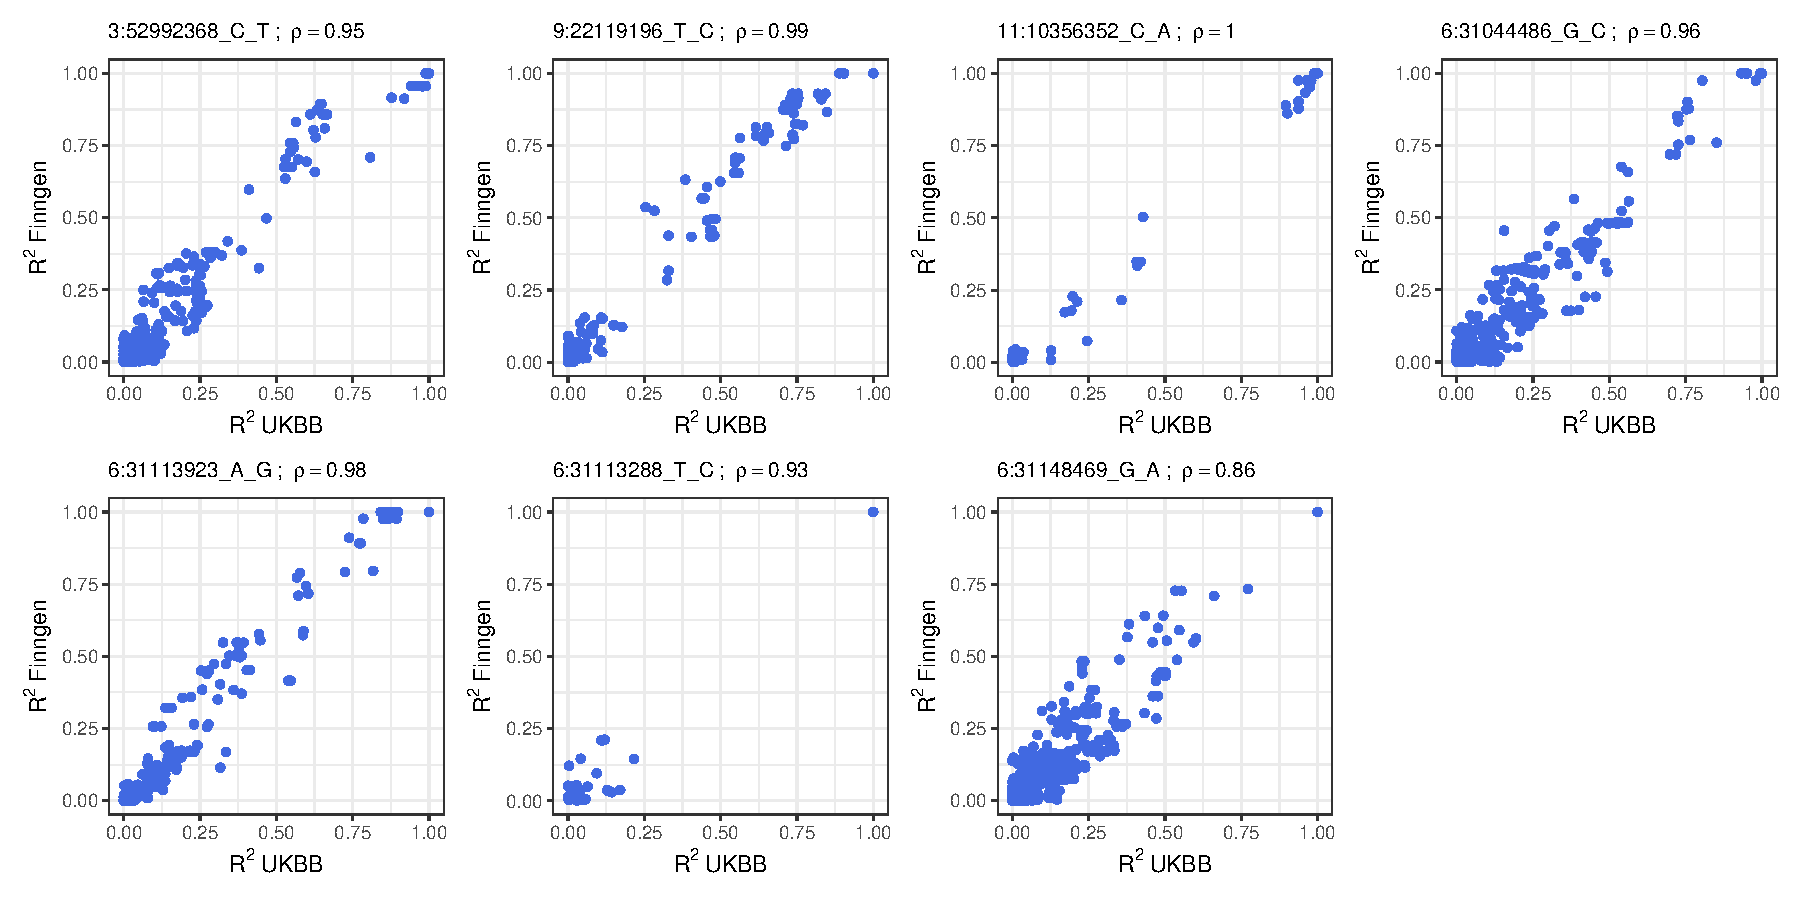
\includegraphics[width=1.0\textwidth]{ukbb_finngen_ld_plot}
%   \caption[Figure]{$R^{2}$ between variants and the index variant in the four pAD-associated loci in non-Finnish Europeans (x-axis) and Finnish Europeans (y-axis). $R^{2}$ values are derived from the 1000GP. Pearson correlation coefficients and index variants are indicated on top of each figure.}
%   \label{fig:ukbb_finngen_ld_plot}
%   \end{figure}

\begin{figure}[H]
  \centering
  \begin{subfigure}[b]{1.0\textwidth}
      \centering
      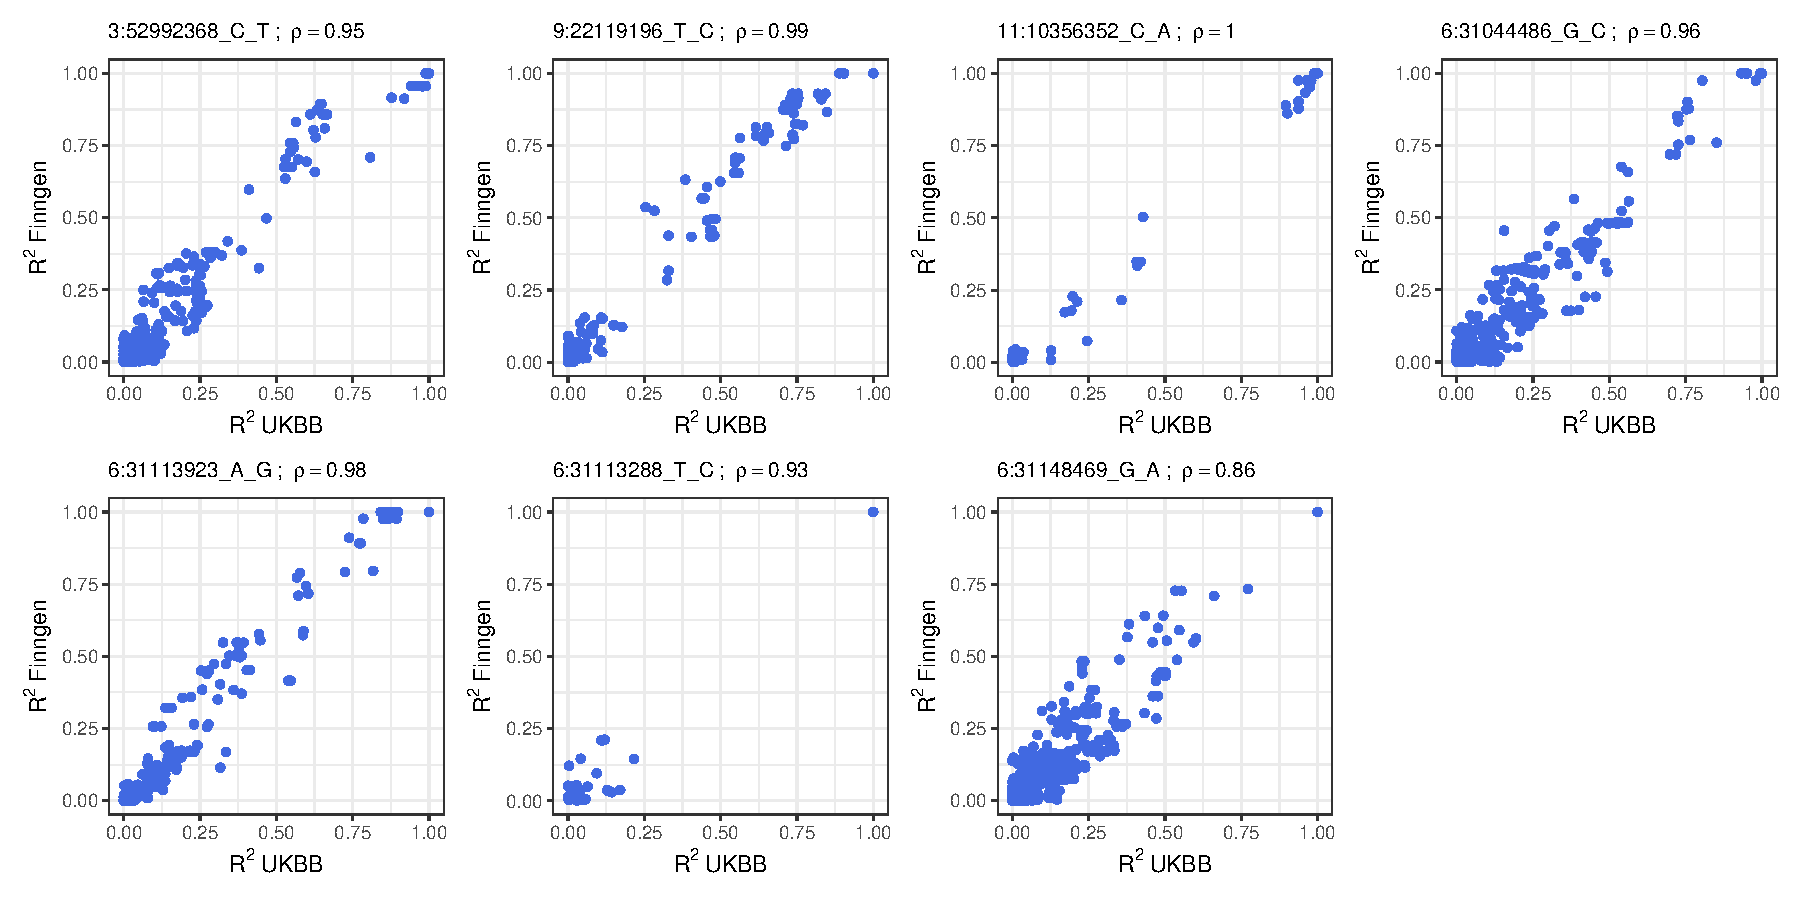
\includegraphics[width=\textwidth]{ukbb_finngen_ld_plot}
      \caption{}
      \label{fig:ukbb_finngen_ld_plot}
  \end{subfigure}
  \hfill
  \begin{subfigure}[b]{1.0\textwidth}
      \centering
      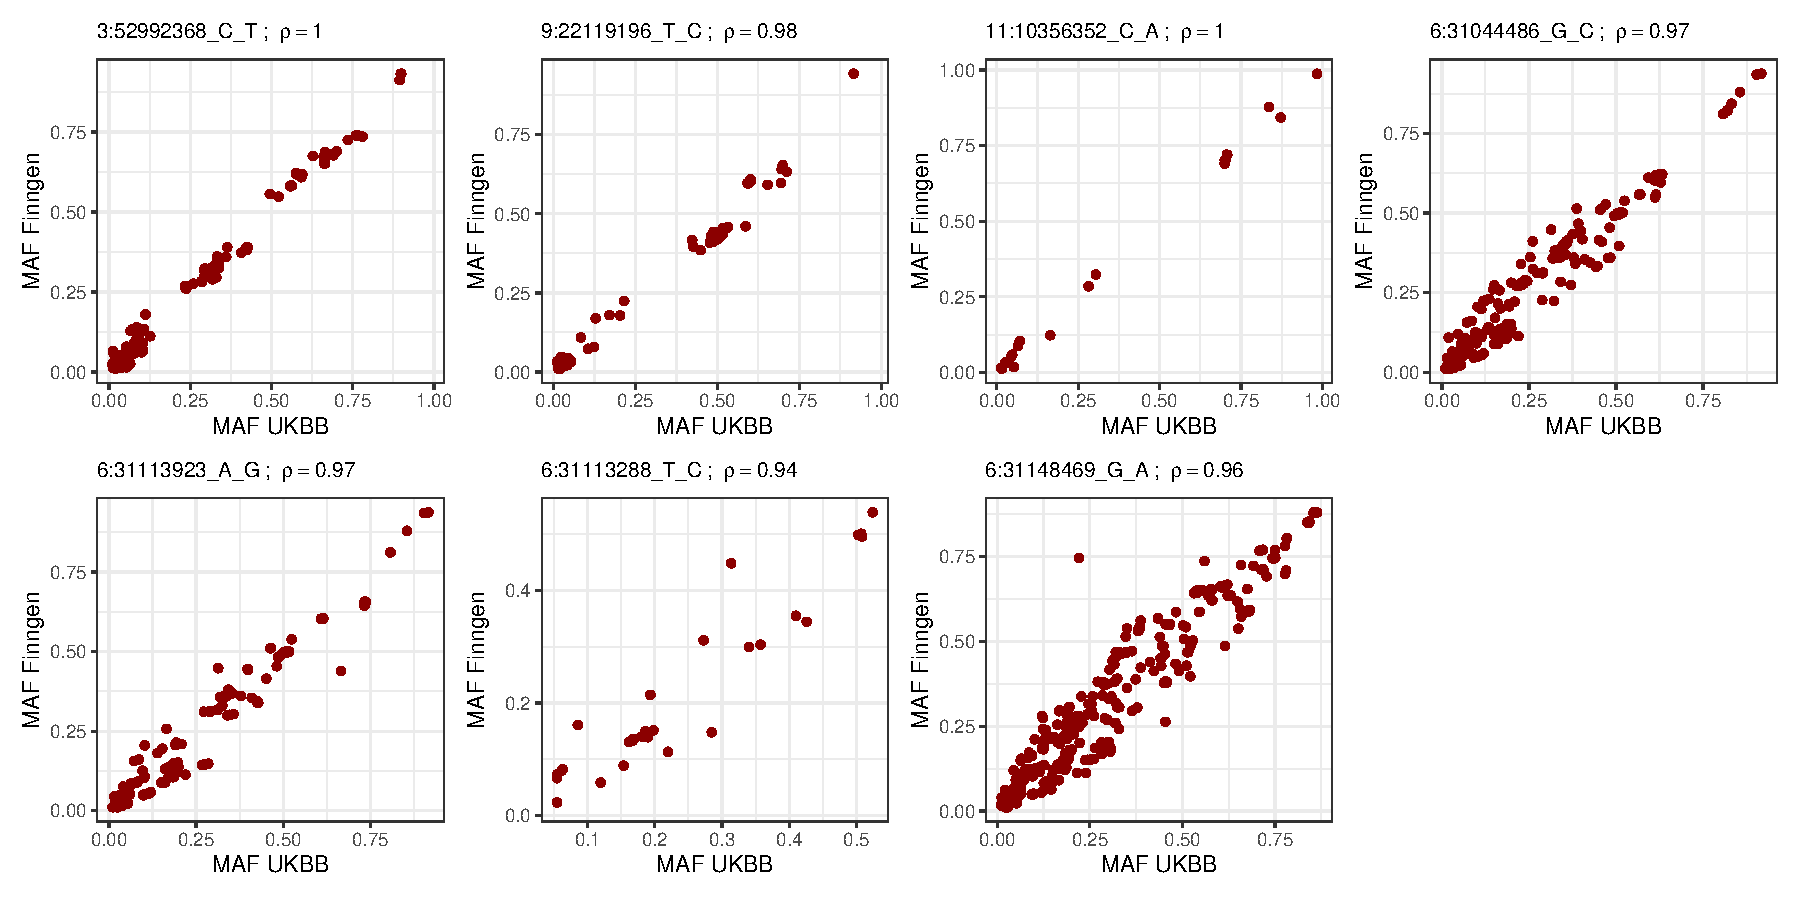
\includegraphics[width=\textwidth]{ukbb_finngen_maf_plot}
      \caption{}
      \label{fig:ukbb_finngen_maf_plot}
  \end{subfigure}


     \caption{(a) $R^{2}$ between variants and the index variant in the four pAD-associated loci in non-Finnish Europeans (x-axis) and Finnish Europeans (y-axis). $R^{2}$ values are derived from the 1000GP. Pearson correlation coefficients and index variants are indicated on top of each figure. (b) MAF of all variants in the UKBB (x-axis) and Finngen (y-axis).}
     \label{fig:tss_esqtl}
\end{figure}
I found that MAF was nearly perfectly correlated in NFE and FE in all seven pAD-associated loci ($\rho$ > 0.94; Figure a). $R^{2}$ were also strongly correlated in all loci ($\rho$ > 0.86;Figure b). Notably, despite a strong $R^{2}$ correlation, 6:31113288\_T\_C did not have any LD friends in FE, similar to GBR and NFE. The strong correlation was driven by variants with a low $R^{2}$ with the index variant. Overall, witht the exception of 6:31113288\_T\_C which did not have any LD friends in FE, both MAF and the LD structure were consistent across all pAD-associated between NFE and FE. Replication of UKBB hits can therefore be reasonably assessed in the Finngen GWAS.\\

\subsubsection{UKBB non-MHC loci replicate in Finngen}
To test the replication of the UKBB hits, I adopted an approach that takes into account differences in LD between FE and NFE. UKBB index variants may not necessarily tag the true causal variants in FE, and an absence of replication of the UKBB index variants in Finngen does not therefore indicate the lack of association at pAD-associated loci. Therefore, I performed the replication using UKBB index variants and all their LD friends in Finngen (R${2}$ > 0.5 in FE). I found that all non-MHC loci replicated (Bonferroni-corrected P-value < $7\times10^{-3}$). Additionally, all top variants in Finngen were in high LD with the UKBB index variants ($R^{2}$ > 0.86). Conversely, none of the MHC loci replicated in Finngen. There are two possible explanations for the absence of replication. First, it is possible that neither the index variants nor their LD friends tag the true causal variant in FE. This is likely to be the case for the MHC loci where the index variant tags several LD friends, but none of them pass the replication P-value threshold. Second, a lack of statistical power might lead to an absence of replication, especially given the heterogeneity in pAD cases. The UKBB pAD case cohort is composed of perianal fissure and fistula cases in roughly equal proportions, but it is unclear if the Finngen case cohort composition is similarly balanced. 

\begin{table}[H]
  \centering
  \begin{tabular}[t]{llllr}
  \toprule
  UKBB & Finngen & P-value UKBB & P-value Finngen & $R^{2}$\\
  \midrule
  3:52992368\_C\_T & 3:53056474\_C\_T & 1.5e-08 & 3.4e-04 & 0.96\\
  6:31044486\_G\_C & 6:31044486\_G\_C & 2.2e-08 & 5.7e-02 & 1.00\\
  6:31113923\_A\_G & 6:31113923\_A\_G & 3.2e-08 & 3.9e-02 & 1.00\\
  6:31113288\_T\_C & 6:31113288\_T\_C & 1.1e-08 & 1.5e-01 & 1.00\\
  6:31148469\_G\_A & 6:31148469\_G\_A & 2.6e-08 & 9.9e-01 & 1.00\\
  \addlinespace
  9:22119196\_T\_C & 9:22090936\_C\_T & 2.7e-08 & 1.5e-03 & 0.86\\
  11:10356352\_C\_A & 11:10363421\_G\_A & 7.3e-09 & 1.7e-07 & 0.98\\
  \bottomrule
  \end{tabular}
  \end{table}

  \subsection{Replication of Finngen loci in UKBB}
  Following the same replication approach, I tested the replication of Finngen's three genome-wide significant loci in the UKBB. For each of the three index variants, I identified all their LD friends in the UKBB, using $R^{2}$ values derived from 1000GP NGE. Then I tested if any of the LD friends show evidence of replication. I found evidence of replication for all three loci in the UKBB (Bonferroni-corrected P-value < 0.017).

  \begin{table}[H]
    \centering
    \begin{tabular}[t]{llllr}
    \toprule
    Finngen & UKBB & P-value Finngen & P-value UKBB & $R^{2}$\\
    \midrule
    1:39817036\_C\_T & 1:39809417\_A\_T & 7.2e-10 & 2.3e-07 & 0.74\\
    6:1771278\_C\_T & 6:1775480\_A\_T & 6.7e-09 & 4.7e-05 & 0.91\\
    12:114235969\_T\_C & 12:114247766\_A\_G & 7.0e-09 & 4.5e-04 & 0.74\\
    \bottomrule
    \end{tabular}
    \end{table}


    \subsection{Meta-analysis}
    Meta-analyisis between GWAS cohorts is commonly used to increase statistical power to identify genome-wide significant loci. Practically, meta-analysis is carried out when the are constraints on sharing individual-level data, or when genotype data from several studies cannot be combined. In these cases, meta-analysis of association summary statistics is the preferred analytical approach, and there is ample evidence that it achieves similar statistical power as combining genotype data from several studies. 

    Several factors affect the effectiveness of genome-wide meta-analyses, including genetic factors as well as factors related to the pAD case cohort. First, Finnish Europenas were admixed with several Central Asian and East Asian populations, as well as Non-Finnish Europeans \cite{Qin2015-jb}. Over the last several thousand years, this admixture led to systematic differences between Finnish and Non-Finnish Europeans, both in terms of allele frequencies and LD strucure.  In addition, local subpopulation stratification in both cohorts may drive spurious associations, which might be amplified in a meta-analysis if not properly accounted for. Second, it is unclear how similar the definition of pAD cases between the two cohorts is similar. Although case and control inclusion criteria are similar between the two cohorts, it is unknown if the composition of the pAD case cohort is similar. Similar to the ICD-10 code used in the UKBB analysis to identify anal fissures and fistula cases, the corresponding FinnGen's clinical endpoint covers several clinical diagnosis. I have shown that the poroption of anal fissures and fistula cases in UKBB are roughly equal withing the pAD case cohort. Since FinnGen's individual-level data are not publicly available, I could not confirm if the proportion of anal fissure and fistula cases are similar. Moreover, it is unclear if FinnGen's case cohort is enriched in any other clinical endpoints compared to FinnGen's control cohort. Showing that the pAD cases are enriched in certain disorders can serve as an important phenotypic quality control check to ensure that both cohorts are as homogenous as possible, and maximises the ability of a meta-analysis to identify genetic variants associated with pAD risk.

    \subsubsection{Meta-analysis and identification of genome-wide significant loci}
    I performed a fixed-effects meta-analysis between UKBB and Finngen summary statistics using effect size estimates and standard errors using METAL. After filtering out variants with MAF < 0.01 and with low imputation score (INFO < 0.4), the two GWAS summary statistics had an intersection of 7,663,827 variants that passed quality control and a total of 11,096,129 variants across the two cohorts. Of these, 2,041,145 variants were specific to UKBB and 1,390,527 were specific to FinnGen. Given that 31\% of variants were unique to one of the two GWAS, I did not remove them from their respective summary statistics file. It is important to note, however, that this choice may favour variants that pass QC in both studies. \\

    I used LD clumping to identify genome-wide significant loci, along with index variants. Because I performed a meta-analysis between FE and NFE summary statistics, I used an LD reference panel derived from both NFE and FE in 1000GP (N=525). Using this approach, I identified 17 genome-wide significant loci (P-value < $5\times10^{-8}$). As a post-meta-analysis quality check, I also estimated the heterogeneity of effect sizes between UKBB and FinnGen using Cochran's Q test, which is implemented in METAL. A strong deviation from the null hypothesis that effect sizes are similar can be considered evidence that the effect size estimates are heterogeneous between the two cohorts, indicating uncertainty of the meta-analysed effect size estimate. To this end, I found no evidence of heterogenity for any of the 17 index variants ($P_{het} < 3\times10^{-3}$). However, tests of effect heterogeneity can often be underpowered to detect a singificant difference in effect size estimates between studies, especially when the confidence intervals around effect size estimates are large. Therefore, an abscence of evidence for heterogeneity may also indicate lack of power to find heterogenity between FinnGen and UKBB. This is a particularly important consideration for the the variants that had suggestive $P_{het}$ (< 0.05; index variants: 3:53034026\_C\_T, 5:64868326\_TTTC\_T and 9:22124505\_A\_T; Table). 

    \begin{tabular}[t]{lllllr}
      \toprule
      ID\_b38 & PVAL\_pad.meta & OR\_ukbb & OR\_finngen & OR\_meta & HetPval\\
      \midrule
      1:39809417\_A\_T & 7.4e-15 & 1.13 & 1.14 & 1.14 & 0.84\\
      \addlinespace
      1:39836225\_G\_C & 4.1e-08 & 1.09 & 1.11 & 1.1 & 0.63\\
      \addlinespace
      3:53034026\_C\_T & 7.5e-10 & 1.13 & 1.07 & 1.09 & 0.05\\
      \addlinespace
      5:64868326\_TTTC\_T & 2.0e-08 & 0.89 & 0.94 & 0.92 & 0.05\\
      \addlinespace
      6:1775202\_G\_A & 1.0e-11 & 0.91 & 0.9 & 0.9 & 0.80\\
      \addlinespace
      6:31121854\_C\_T & 4.2e-08 & 1.11 & 1.06 & 1.08 & 0.08\\
      \addlinespace
      6:31253340\_T\_C & 3.8e-08 & 1.1 & 1.07 & 1.08 & 0.24\\
      \addlinespace
      6:133008360\_T\_A & 2.7e-08 & 1.12 & 1.1 & 1.11 & 0.47\\
      \addlinespace
      6:133260944\_G\_A & 4.7e-08 & 1.11 & 1.08 & 1.1 & 0.42\\
      \addlinespace
      6:133267939\_T\_C & 4.5e-08 & 1.09 & 1.07 & 1.08 & 0.42\\
      \addlinespace
      7:2524404\_G\_A & 4.1e-08 & 1.14 & 1.13 & 1.14 & 0.76\\
      \addlinespace
      8:70735125\_A\_G & 3.9e-11 & 0.83 & 0.82 & 0.83 & 0.94\\
      \addlinespace
      8:70993166\_AAGTT\_A & 1.2e-10 & 0.83 & 0.82 & 0.82 & 0.75\\
      \addlinespace
      9:22124505\_A\_T & 2.1e-08 & 0.9 & 0.95 & 0.92 & 0.05\\
      \addlinespace
      10:61661180\_A\_G & 2.0e-08 & 1.09 & 1.08 & 1.09 & 0.90\\
      \addlinespace
      11:10356352\_C\_A & 1.3e-13 & 0.88 & 0.91 & 0.89 & 0.27\\
      \addlinespace
      12:114235969\_T\_C & 4.2e-10 & 1.07 & 1.11 & 1.09 & 0.20\\
      \bottomrule
      \end{tabular}


  %   Why performed meta-analysis? 
  %   \begin{itemize}
      
      
  %     \item \textbf{Pros} 
  %     \item Any concerns about difference in phenotype definitions: 
  %     \item reasons why that might be the case (difference in proporion - biases introduced by different clinical systems - differences in prevalence)
  %     \item Any concerns about differences in LD and MAF and subpopulation stratification and how that was adressed
  %     \item \textbf{Cons}
  %     \item  Maximise in power
  %     \item pop strat can be taken care of by adjusting lambda gc
  %     \item Individual-level data are required for better definition of phenotype
  % \end{itemize}
    
  \subsection{MAF and R2 between Finngen and UKBB at LD friends}
  As a follow-up to the three loci whose index variants showed suggestive evidence of effect size heterogenity ($P_{het}$ < 0.05), I performed two further post-meta-analysis quality checks. First, this discrepancy could be due to a difference in general-population MAF between FE and NFE. 
  \subsection{}
  \subsection{Disentangling the genetic effect of pAD-associated variants on related intestinal disorders}

  In section \ref{section:pheno_enrich}, I analysed the composition of the pAD case cohort and showed that it is significantly enriched with 199 ICD-10 clinical codes compared to pAD controls. I hypothesised that this enrichment was also reflected at the level of genetic risk predisposition. To confirm this, I performed a genetic correlation analysis using LD score regression (LDSC). LDSC is a method that quantifies the shared genetic risk between two traits using only GWAS summary statistics, and is therefore a widely-used method to investigate the genetic relationship between a trait of interest and other related traits without the need to access individual-level data. To this end, I first downloaded GWAS summary statistics from the Pan-UKBB project, a large-scale analysis that performed a UKBB case-control GWAS analysis for 7,228 UKBB phenotypes including all ICD-10 codes. I carried out a genetic correlation analysis between the pAD meta-analysis and the Pan-UKBB haemorrhoids GWAS, and found strong evidence of high genetic correlation (ICD-10 code I84; P-value=$5.37\times10^{-26}$; $r_{g}$=0.66). To validate this correlation, I repeated the genetic correlation analysis using a larger haemorrhoids GWAS of over 900,000 individuals by Zheng et al. 2021 \cite{Zheng2021-ss}. I found a similar genetic correlation estimate that was even more significant than the estimate from the Pan-UKBB analysis ($r_{g}$=0.63; P-value=$10^{-62}$).
  

  The existence of a strong genetic correlation and enrichment of haemorrhoids could be explained by several factors. First, pAD could be a co-morbidity of Haemorrhoids, in a similar way that Type 2 diabetes and obesity are comorbidities. This could be a result of the same risk factors (genetic or otherwise) underlying both diseases, potentially with varying effect sizes. Alternatively, clinical diagnostic factors could also account for this overlap. Both diseases are among the differential diagnoses of patients presenting with rectal pain, swelling, bleeding and discharge. Therefore, a patient suffering from inflammed haemorrhoids is more likely to be diagnosed if they also suffer from pAD (e.g. after performing rectal examination). 

Bias introduced by clinical diagnostic factors cannot be completely addressed with observational data, as this will require constructing pAD case-control cohorts where haemorrhoids cases are either balanced or actively excluded from both cases and controls. However, the impact of such bias could be assessed by performing a pAD GWAS where haemorrhoids cases are excluded from cases and controls (pADexclHaem), and a haemorrhoids GWAS where pAD cases are excluded from cases and controls (HaemexclpAD). Comparing the genetic association effect sizes of the previously reported 17 index variants between pADexclHaem and HaemexclpAD may give an indication as to which genetic variants are likely to underlie both diseases and which are likely to be specific to pAD.

Constructing the two cohort requires access to a individual-level phenotypic data in both UKBB and Finngen. Therefore, I tested the hypothesis that effect sizes are different between the haemorrhoids and pAD in the UKBB only. To construct the HaemexclpAD case and control cohorts, I selected individuals who have been diagnosed with ICD-10 code I84 or ICD-9 code 455 in at least one inpatient visit as cases and excluded individuals with ICD-10 code K60 or ICD-9 code 565 from both cases and controls. Similarly, for pADexclHaem, I selected individuals who have been diagnosed with ICD-10 code K60 or ICD-9 code 565 in at least one hospital visit and excluded individuals with ICD-10 code I84 or ICD-9 code 455 from both cases and controls. Additionally, I applied the same control exclusion criteria in Table \ref{table:ukbb_ctrl_excl_criteria}. 

\begin{figure}[H]
  \centering    
  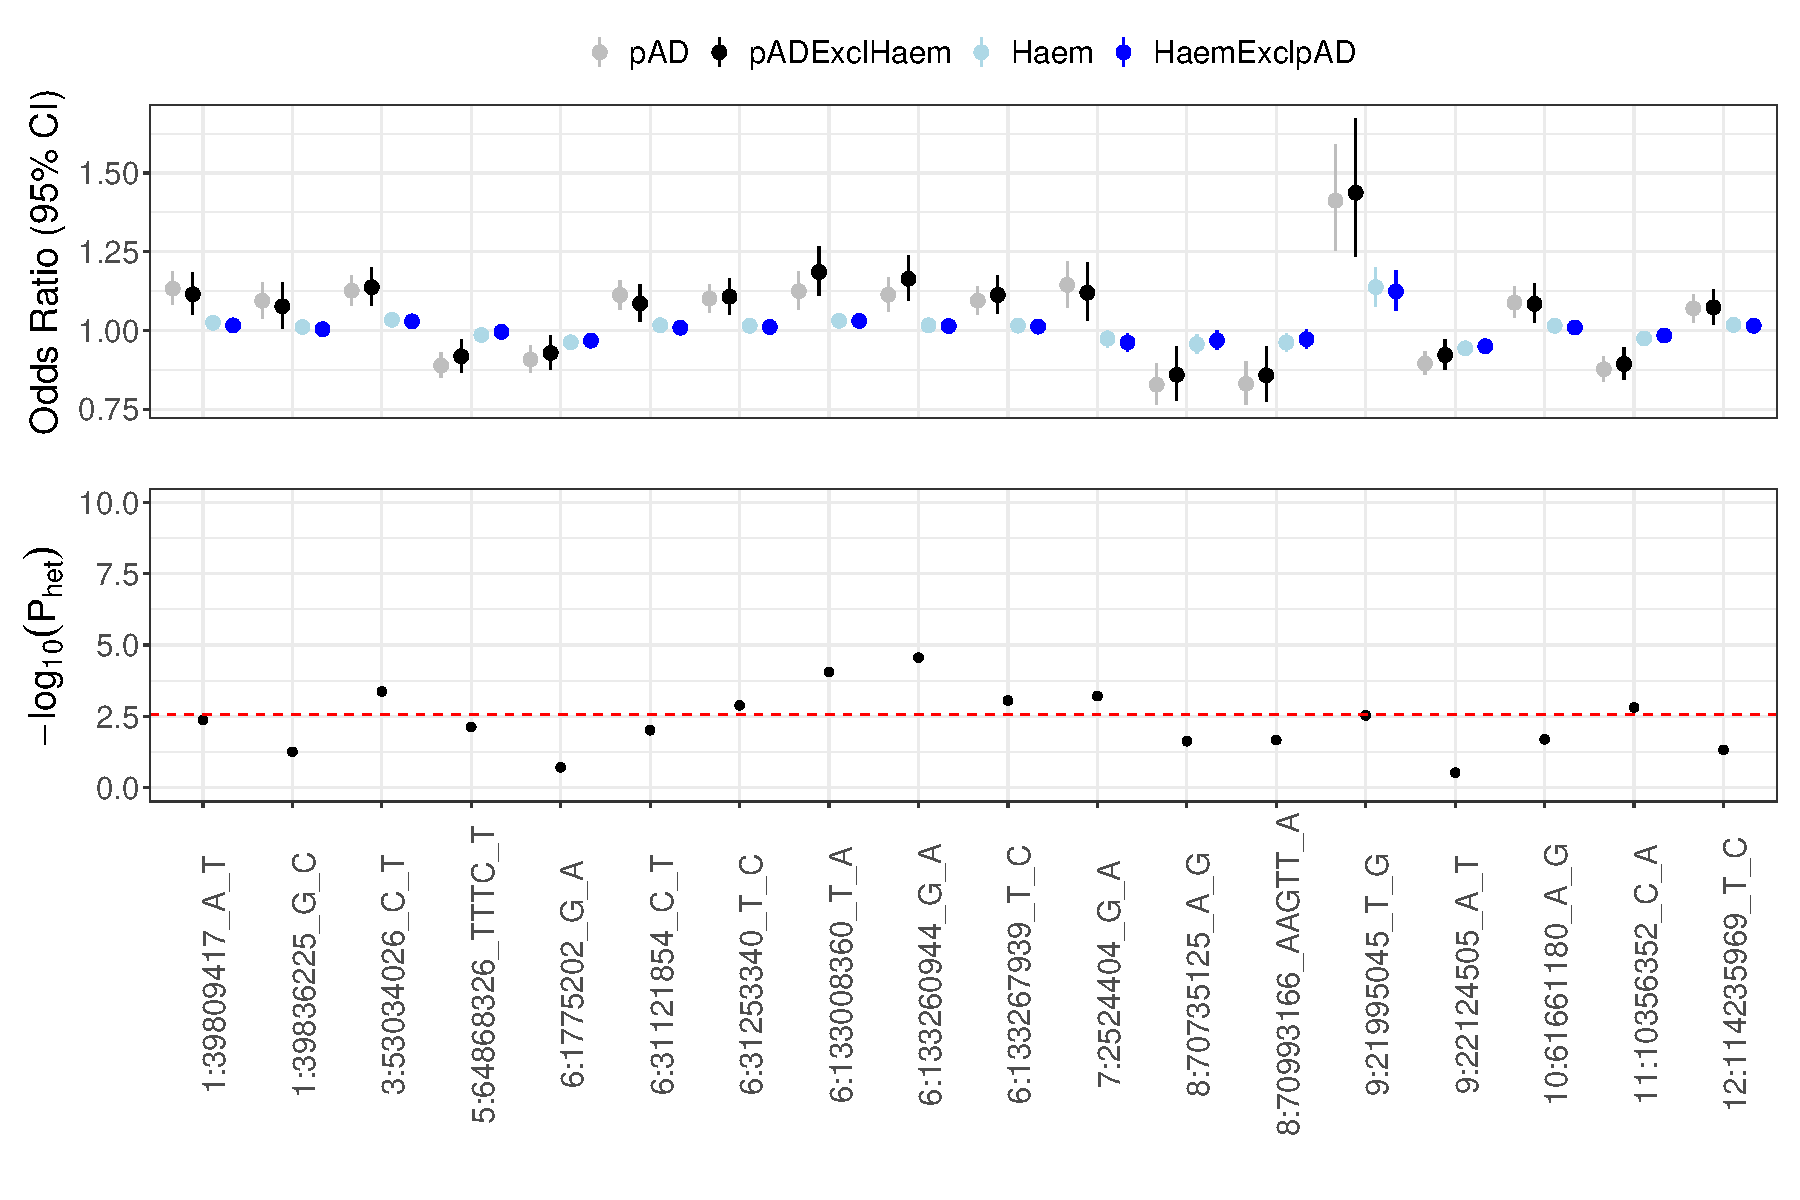
\includegraphics[width=1.0\textwidth]{combined_forest_het_plt}
  \caption[Figure]{Top plot shows the ffect sizes of the 17 pAD-assocaited index variants from four UKBB case/control cohorts: pAD in grey ($N_{case}$=4,606), pADExclHaem in black ($N_{case}$=2,799), Haem in light blue ($N_{case}$=29,285), and HaemExclpAD in blue ($N_{case}$=27,477). Bottom plot shows the heterogeneity of effect-size P-value ($P_{het}$) between the two disjoint GWAS analyses: pADExclHaem and HaemexclpAD. The red dotted line shows $P_{het}$ significance threshold ($P_{het} < 3\times10^{-3}$).}
  \label{fig:combined_forest_het_plot}
  \end{figure}

I tested the association of each of the 18 pAD-associated index variants with each of the four phenotypes described above. First, I examined if any of the index variants were associated with the two haemorrhoids phenotypes Haem and HaemExclpAD. Since I performed a targeted association test, I set a more permissive assocition threshold for declaring significance than normally used to declare genome-wide assoctions (P < $3\times10^{-3}$). Despite the large difference in statistical power between the two haemorrhoids cohorts and the two pAD cohorts, I found that only four of the tested index variants achieved significant association with haemorrhoids (index variants: 3:53034026\_C\_T, 6:1775202\_G\_A, 9:21995045\_T\_G and 9:22124505\_A\_T). Additionally, all four variants were significant in both Haem and HaemExclpAD, suggesting that the exclusion of pAD cases from the haemorrhoids cohort has little impact on their association. Additionally, 3:53034026\_C\_T showed significant evidence of effect size heterogeneity between pADExclHaem and HaemExclpAD ($P_{het}$ < $3\times10^{-3}$; Figure \ref{fig:combined_forest_het_plot}), with a significantly larger effect on pADExclHaem($OR_{pADExclHaem}=1.14-1.2$ and $OR_{HaemExclpAD}=1.03-1.05$).

Although the rest of the 18 index variants did show a significant association with the two haemorrhoids definition, I observed a pattern similar to 3:53034026\_C\_T. Seven of the 18 pAD-associated index variants had significantly smaller effect sizes in HaemexclpAD than in pADexclHaem ($P_{het}$ < $3\times10^{-3}$; Figure \ref{fig:combined_forest_het_plot}). Moreover, 8 additional variants had suggestive evidence of heterogeneity of effect ($P_{het}$ < 0.05), and in all cases the effect size was larger in pADExclHaem than in HaemExclpAD. 

Two conclusion can be made from this analysis. First, despite a much larger sample size in favour of the haemorrhoids cohorts, only four pAD-associated index variants were also associated with haemorrhoids, even with a relatively lenient threshold for association. Second, despite their nominal association with haemorrhoids, these four variants (and indeed all other variants) had a consistently smaller effect size on HaemExclpAD than pADExclHaem, and for 3:53034026\_C\_T that difference in effect size was significant. More importantly, this pattern was observed for all 18 index variants, despite the lack of power to detect a significant heterogeneity of effects. Performing a similar 'disentaglment' analysis in both Finngen and UKBB, and subsequently identifying which variants have a significantly larger effect size in pADExclHaem than HaemExclpAD is a plausible way to validate this pattern. Such validation would conclusively establish those variants as bona fidae pAD-associated variants.\\



\subsection{Colocalisation analysis}
Many GWAS loci that have been uncovered over the last 15 years are located in non-coding regions. This complicates the task of understanding their downstream effects and linking them to effector genes. Over the last ten years, large-scale studies that map genetic variants associated with transcriptomic variation have improved our understanding of the downstream effects of disease-associated genetic variants. For example, the Gentype Expression Project (GTEx) has mapped genetic variants associated with individual variation in overall levels of gene expression (eQTL) and splicing (sQTL). Additionally, statistical methods that are able to integrate association signals from different studies have been applied to GWAS and QTL data in order to investigate which effector genes likely underpin disease-associated GWAS signals. Colocalisation analysis, for example, quantifies the probability that two association signals are driven by a single causal variant ($PP_{4}$) and can therefore be used to compare GWAS and QTL association signals.\\

I carried out colocalisation analysis between the 18 pAD-associated loci and eQTL and sQTL signals from GTEx v8. I colocalised each of the 18 loci with all eQTLs and sQTLs in a 1 mbp window centered around each locus' index variant. Across all 49 GTEx tissues, I performed the colocalisation with a total of 519 genes and all their splice junctions (see Methods for the number of genes and splice junctions tested for each locus). The most informative output of colocalisation analysis is $PP_{4}$, the posterior probability of two association signals sharing a single underlying variant. Overall, I found high-confidence colocalisation evidence for 8 loci, where at least one eQTL or sQTL colocalised with each pAD-associated locus ($PP_{4}$ > 0.8; Table \ref{table:coloc_res}). All 8 loci had at least a single colocalisation with an sQTL (16 sQTL genes), while 6 loci colocalised with at least one eQTL signal (10 eQTL), implicating a total of 21 genes. In many cases where both an eQTL and sQTL colocalisation were detected, distinct eQTL and sQTL genes were implicated. Moreover, different tissues often implicated different genes. For example, the locus at index variant 7:2524404\_G\_A colocalised with two different QTL genes (\textit{BRAT1} in the liver and thyroid gland, and \textit{LFNG} in the skin and whole blood). In fact, 4 of the 8 colocalised loci implicated a single gene, and only two loci implicated the same gene with high confidence in multiple tissues (index variant 10:61661180\_A\_G and 5:64868326\_TTTC\_T). The pleiotropic nature of genetic effects on gene expression is well documented in GTEx \cite{Ribeiro2021-xj}, and even in other organisms \cite{Brem2002-zj,Schadt2003-ei}. This pleiotropy is often attributed to the widespread gene co-expression patterns, whereby the expression of multiple genes is controlled by a single locus, sometimes termed "eQTL hotspots" \cite{Tian2016-hy}. Co-expressed genes are often found to be functionally related via shared biological pathways \cite{Van_Dam2017-vm,Westra2013-mm}. To explore this, I performed a gene set enrichment analysis in four databases: Reactome \cite{Gillespie2022-jr}, the Gene Ontlogy (GO) Molecular Function database, GO Cellular Component and GO Biological processes \cite{Thomas2022-nb}. I did not find any significantly enriched pathways in any of the the three GO databases or the Reactome database. Notably, 8 of the 21 genes were not found in the Reacome database, reflecting the lack of knowledge of their biological functions. 

\begin{longtable}[t]{l>{\raggedright\arraybackslash}p{10em}>{\raggedright\arraybackslash}p{10em}}
  \caption{shows}
    \label{table:coloc_res}\\
    \hline
  \toprule
  Index SNP & Tissues (eQTL) & Tissues (sQTL)\\
  \midrule
  \endfirsthead
  \caption[]{ \textit{(continued)}}\\
  \toprule
  Index SNP & Tissues (eQTL) & Tissues (sQTL)\\
  \midrule
  \endhead
  
  \endfoot
  \bottomrule
  \endlastfoot
  \begingroup\fontsize{9}{11}\selectfont 1:39809417\_A\_T\endgroup & \begingroup\fontsize{9}{11}\selectfont NA\endgroup & \begingroup\fontsize{9}{11}\selectfont Brain Amygdala (PPIE: 0.85), Testis (PPIE: 0.82), Thyroid (PPIEL: 0.82), Brain Anterior cingulate cortex BA24 (PPT1: 0.86), Nerve Tibial (TRIT1: 0.83), Testis (TRIT1: 0.86)\endgroup\\
  \midrule
  \begingroup\fontsize{9}{11}\selectfont 1:39836225\_G\_C\endgroup & \begingroup\fontsize{9}{11}\selectfont NA\endgroup & \begingroup\fontsize{9}{11}\selectfont Brain Amygdala (PPIE: 0.85), Testis (PPIE: 0.82), Thyroid (PPIEL: 0.82), Brain Anterior cingulate cortex BA24 (PPT1: 0.86), Nerve Tibial (TRIT1: 0.83), Testis (TRIT1: 0.86)\endgroup\\
  \midrule
  \begingroup\fontsize{9}{11}\selectfont 3:53034026\_C\_T\endgroup & \begingroup\fontsize{9}{11}\selectfont Kidney Cortex (ITIH4: 0.97), Colon Transverse (SFMBT1: 0.98), Esophagus Gastroesophageal Junction (SFMBT1: 0.95), Esophagus Muscularis (TMEM110: 0.82), Pancreas (TMEM110: 0.98)\endgroup & \begingroup\fontsize{9}{11}\selectfont Artery Aorta (ITIH4: 0.9), Artery Tibial (ITIH4: 0.97), Liver (ITIH4: 0.96), Nerve Tibial (ITIH4: 0.93), Liver (MUSTN1: 0.87), Esophagus Muscularis (RFT1: 0.84)\endgroup\\
  \midrule
  \begingroup\fontsize{9}{11}\selectfont 5:64868326\_TTTC\_T\endgroup & \begingroup\fontsize{9}{11}\selectfont Testis (CWC27: 0.86)\endgroup & \begingroup\fontsize{9}{11}\selectfont Esophagus Muscularis (CWC27: 0.81), Testis (CWC27: 0.84)\endgroup\\
  \midrule
  \begingroup\fontsize{9}{11}\selectfont 6:31121854\_C\_T\endgroup & \begingroup\fontsize{9}{11}\selectfont Lung (HLA-B: 0.86), Thyroid (HLA-B: 0.87), Adrenal Gland (POU5F1: 0.85), Brain Cerebellar Hemisphere (POU5F1: 0.89), Brain Cerebellum (POU5F1: 0.91), Brain Hypothalamus (POU5F1: 0.84)\endgroup & \begingroup\fontsize{9}{11}\selectfont Skin Not Sun Exposed Suprapubic (FLOT1: 0.85), Skin Not Sun Exposed Suprapubic (MICA: 0.81), Colon Transverse (PSORS1C1: 0.98), Lung (PSORS1C1: 0.99), Small Intestine Terminal Ileum (PSORS1C1: 0.89)\endgroup\\
  \midrule
  \addlinespace
  \begingroup\fontsize{9}{11}\selectfont 6:31253340\_T\_C\endgroup & \begingroup\fontsize{9}{11}\selectfont Lung (HLA-B: 0.86), Thyroid (HLA-B: 0.87), Adrenal Gland (POU5F1: 0.85), Brain Cerebellar Hemisphere (POU5F1: 0.89), Brain Cerebellum (POU5F1: 0.91), Brain Hypothalamus (POU5F1: 0.84)\endgroup & \begingroup\fontsize{9}{11}\selectfont Skin Not Sun Exposed Suprapubic (MICA: 0.81), Colon Transverse (PSORS1C1: 0.98), Lung (PSORS1C1: 0.99), Small Intestine Terminal Ileum (PSORS1C1: 0.89)\endgroup\\
  \midrule
  \begingroup\fontsize{9}{11}\selectfont 7:2524404\_G\_A\endgroup & \begingroup\fontsize{9}{11}\selectfont Liver (BRAT1: 0.94), Skin Not Sun Exposed Suprapubic (LFNG: 0.92), Skin Sun Exposed Lower leg (LFNG: 0.99), Whole Blood (LFNG: 0.85)\endgroup & \begingroup\fontsize{9}{11}\selectfont Thyroid (BRAT1: 0.95), Skin Not Sun Exposed Suprapubic (LFNG: 0.86), Skin Sun Exposed Lower leg (LFNG: 0.95), Whole Blood (LFNG: 0.99)\endgroup\\
  \midrule
  \begingroup\fontsize{9}{11}\selectfont 10:61661180\_A\_G\endgroup & \begingroup\fontsize{9}{11}\selectfont Minor Salivary Gland (C10orf107: 0.96)\endgroup & \begingroup\fontsize{9}{11}\selectfont Brain Anterior cingulate cortex BA24 (C10orf107: 0.81), Testis (C10orf107: 0.9)\endgroup\\
  \midrule
  \begingroup\fontsize{9}{11}\selectfont 11:10356352\_C\_A\endgroup & \begingroup\fontsize{9}{11}\selectfont NA\endgroup & \begingroup\fontsize{9}{11}\selectfont Adrenal Gland (AMPD3: 0.85)\endgroup\\
  \midrule
  \begingroup\fontsize{9}{11}\selectfont 12:114235969\_T\_C\endgroup & \begingroup\fontsize{9}{11}\selectfont NA\endgroup & \begingroup\fontsize{9}{11}\selectfont Vagina (RBM19: 0.81)\endgroup\\*
  \end{longtable}

  Only a single locus implicated a single gene across various tissues and with both eQTL and sQTL colocalisation evidence (\textit{CWC27}; index variant 5:64868326\_TTTC\_T; $PP_{4}$ > 0.8). The protective allele of the index variant (odds ratio=0.91) increases the expression of CWC27 (eQTL effect size=0.29), and also changes usage of five CWC27 splice junctions in testis. All implicated splice junctions are located within intron 11-12 of CWC27. CWC27 codes for a protein that forms part of the splicesome, a complex machinery that  which is part of a complex Rare CWC27 variants are known to be associated with retinitis pigmentosa with or without skeletal symptoms. Xu et al. [ref] performed whole-exome sequencing of ten individuals from seven unrelated families, nine of which suffered from retinitis pigmentosa, either alone or with a range of structural disorders such as bradydactyly, short stature, and craniofacial defects. In all seven families, rare protein-truncating variants in CWC27 were found, establishing CWC27 as the effector gene for this group of rare disorders. 



\section{Methods}
\subsection{UKBB GWAS using REGENIE}
Explain REGENIE - which version - say what you did to account for case/control imbalance and explain pFirth - 
\subsection{Defining GWAS loci}
I defined genome-wide significant loci from GWAS summary statistics using PLINK v1.9 via a clumping procedure. Briefly, clumping represents genome-wide significant loci using the most significant association (termed index variant). It then proceeds to define a locus by clumping neighbouring correlated variants. Specifically, any variants within a predefined window that are correlated with the index variant are considered to belong to the same locus represented by the index variant (i.e. variants in high LD). I used VCFs downloaded from the 1000 Genomes Project High Coverage, which I used compute LD, and set a maximum P-value of $5\times10^{-8}$ for defining a genome-wide significant locus, with default values for the rest of the parameters: variants with $R^{2}$ < 0.5, variants outside a window of 250 kbp, or variants that have a P-value > 0.01 are not clumped with the index variant.
\begin{verbatim}
  plink --clump-p1 0.00000005 --clump-r2 0.50 --clump-kb 250 
  --clump-p2 0.01
\end{verbatim}

PLINK outputs each locus' index variant along with any variants that meet the clumping criteria outlined above. I then defined each locus' boundaries by sorting the clumped variants within each locus according to their genomic location: the most downstream variant defined the 5' boundary and the most upstream variant defined the 3' boundary. 

\subsection{LD calculation from 1000GP}
In order to assess the relationship between the association strength and LD in genome-wide significant loci, I computed LD from 1000GP. I downloaded VCFs from the 1000GP high coverage and used PLINK v1.9 to compute LD between all variants and the index variant at each locus. For each GWAS check I used individuals assigned to the relevant reference population: NFE for UKBB and FE for Finngen.
\begin{verbatim}
  plink --r2 --keep EUR.samples --ld-window-r2 0 
\end{verbatim}

\subsection{Finngen summary statistics preprocessing}
Publicly available Finngen GWAS summary statistics (data freeze 7) were downloaded from the Finngen results website \Verb+finngen.fi/en/access_results+. Similar to UKBB, variants with MAF < 0.01 were removed, but imputation quality information were not available, so I was not able to filter out variants with low imputation quality. 

\subsection{Meta-analysis of UKBB and Finngen}
I used METAL to perform the meta-analysis between UKBB and FinnGen GWAS summary statistics.  METAL can perform fixed-effects meta-analysis using one of two different well-established schemes: P-values and effective sample size, or effect sizes and standard errors. The P-value scheme is implemented to enable meta-analysis of GWAS summary statistics that do not report the effect allele, while the effect sizes scheme can be used when each variant's effect size and effect allele are reported. Both my UKBB analysis and FinnGen's summary statistics report the effect allele, I used the effect size scheme of METAL (\Verb+SCHEME STDERR+). \\

Moreover, METAL automatically aligns any variants that may be flipped between the meta-analysed summary statistics. METAL also enables filtering of variants to be meta-analysed based on their allele frequencies, which was not necessary since I previously filter out variants with MAF < 0.01 in each summary statistics file. Finally, given the differences, allele frequencies, and potential subpopulation stratification between the FinnGen and UKBB GWAS, I enabled a METAL option to correct genomic inflation before performing the meta-analysis (\Verb+GENOMICCONTROL ON+) as recommended in METAL's documentation website. There was no evidence of genomic inflation in the meta-analysed summary statistics ($\lambda_{GC}$=1.024).\\

For each variant, METAL outputs the effect allele, meta-analysed effect size, standard error, and P-values. After performing meta-analyses, it is important to compare the effect sizes between the meta-analysed cohorts. Comparison of both the direction and magnitude of effect sizes gives an indication on how similar the estimated effects of meta-analysed genetic variants are. To formally test this, METAL uses Cochran's Q test to test for effect size heterogeneity. Cochran's Q test asseses two or more effect size estimates and their corresponding standard errors and reports a $\chi^{2}$ statistic that quantifies the deviation from the null hypothesis that the meta-analysed effect sizes are similar. Depending on the number of meta-analysed studies (in this case 2), a P-value is derived from a theoretical $\chi^{2}$ distribution with $N-1$ degrees of freedom, where N is the number of meta-analysed studies (heterogeneity of effect P-value $P_{het}$). I used $P_{het}$ to test if index variants at genome-wide significant loci demonstrate heterogeity of effect size between the two cohorts. To account for multiple index variants being tested, I set a Bonferroni-coorected P-value threshold for rejecting the null hypothesis that the effect sizes are significantly different between the two studies (P-value < $\frac{0.05}{k}$, where $k$ is the number of genome-wide significant variants).


\subsection{Phenotype enrichment analysis}
Explain which ICD codes you tested - explain that you didn't apply coontrol exclusion criteria - explain how you performed Fisher's exact test and which R function you used
\subsection{Genetic correlation analysis}
Genetic correlation analysis is commonly employed to understand the genetic similarities between two phenotypes or diseases of interest. Linkage disequillibrium score regression (LDSC \cite{Bulik-Sullivan2015-fk}) leverages association summary statistics between a pair of traits to compute a genetic correlation estimate ($r_{g}$). The availability of GWAS summary statistics for large numbers of traits and diseases makes genetic correlation a feasible exploratory analysis to discover genetic similarities between traits.\\

The fundamental concept of LDSC is that there is a linear relationship between the Z-score product ($z_{1}z_{2}$) and the LD score of SNPs, where LD score is defined as the sum of $R^{2}$ values for all SNP in a pre-defined windown (the default is 1 cM) \cite{Bulik-Sullivan2015-ts}. The rationale behind this relationship is that SNPs with a higher LD score are more likely to tag the causal variant at each locus, and will therefore have a larger $z_{1}z_{2}$ value. Regressing the LD score for all SNPs can give an estimate of the overall genetic covariance between two traits.Specifically, the regression slope quantifies the gentic covariance, which can then be normalised by the sample sizes of the two traits and the number of SNPs to obtain a genetic correlation estimate between the two traits ($r_{g}$).\\

The accuracy of $r_{g}$ rests on the assumption that the GWAS populations match the LD scores population. By default, LD scores are provided by LDSC, which are computed from the HapMap3 European-ancestry reference panel \cite{hapmap}. It is also important to note that although $r_{g}$ is a genome-wide measure, its computation is based on a predefined set of SNPs. The estimation of $r_{g}$ is based on a set of high-quality common SNPs in HapMap3, which is also provided by LDSC (MAF $\geq$ 0.05; N=1,217,312).

\subsubsection{Genetic correlation between pAD and haemorrhoids}
I used LDSC to compute $r_{g}$ between my pAD meta-analysis and two haemorrhoids GWASes (Zheng et al. 2021 \cite{Zheng2021-ss} and the Pan-UKBB GWAS: \Verb+pan.ukbb.broadinstitute.org/+). I downloaded the Zheng et al. 2021 summary statistics via the GWAS catalogue website (study accession: GCST90014033; $N_{cases}$=218,920; $N_{controls}$=725,213). Since the Pan-UKBB performed the haemorrhoids GWAS using different ancestries, I used the summary statistics from the European-ancestry GWAS only (ICD-10 code: I84; $N_{cases}$=26,348; $N_{controls}$=394,183). \\

After downloading the two haemorrhoids summary statistics, I preprocessed both of them using the LDSC script \Verb+munge_sumstats.py+. The script filters the SNPs and aligns their alleles to the HapMap3 SNP list using the flag \Verb+--merge_alleles hm3.snplist+. This script also takes as input a signed summary statistic column which I provided using the flag \Verb+--signed-sumstats effect_size,0+, where the first argument specifies the column name (effect size column) and the second argument specifies the expected value of the signed summary statistic. Each of the two "munged" summary statistics files were then provided as input to the \Verb+ldsc.py --rg+, along with the pAD summary statistics file, and $r_{g}$ is then computed between pAD and each of the two haemorrhoids GWASes. 


\subsection{Colocalisation analysis}
In order to link the meta-analysis genome-wide significant loci to effector genes, I performed statistical colocalisation with a set of expression and splicing QTLs from the Genotype Excpression Project (GTEx v8). Colocalisation analysis is a statistical approach that uses two summary statistics from two association studies in order to make an inference whether the two association signal are likely to be driven by a shared causal variant. A fundamental assumption of colocalisation is that a single causal variant underlies both association signals under comparison. Under this assumption, five different hypothesis regarding the relationship between the two association signals are tested:
\begin{itemize}
  \item $H_{0}$: none of the two signals are associated with their corresponding traits
  \item $H_{1}$: only the first signal is associated with its corresponding trait
  \item $H_{2}$: only the second signal is associated with it corresponding trait
  \item $H_{3}$: the two signals are associated with their corresponding traits, with different underlying genetic variants
  \item $H_{4}$: the two signals are associated with their corresponding traits, and share a single underlying genetic variant.
\end{itemize}
Certainty about each of these hypotheses is quantified as a posterior probability. Therefore, colocalisation analysis outputs four different posterior probabilities: $PP_{0}$, $PP_{1}$, $PP_{2}$, $PP_{3}$, and $PP_{4}$. Statistical colocalisation is implemented in the R package \Verb+coloc v5.1.2+.

To maximise the ability of \Verb+coloc+ to identify effector genes, I downloaded summary statistics from GTEx v8, a large compendium of expression and splicing quantitative trait loci (eQTLs and sQTLs) mapped from RNA-seq samples obtained from 49 human tissues, ranging in sample sizes from 73-706 individuals. eQTLs and sQTLs were mapped in a 1mbp window around the transcript start site (TSS) of each gene (cis-eQTLs and cis-sQTLs) using genotyped or imputed variants with MAF $\geq$ 0.01.

Within each of the meta-analysis genome-wide significant loci, I identified a list of genes and splice junctions for eQTL and sQTL colocalisation, respectively. To achieve this, for each locus I defined a 1 mbp window around the index variant at each locus, and created a set of genes and splice junction whose respective TSS is located within this window. Next, I performed colocalisation analysis between the meta-analysis summary statistics and each gene's or splice junction's summary statistics. I used the \Verb+coloc.abf()+, which takes as input effect sizes and standard errors of each variant from the meta-analysis and gene or splice junction being tested. Importantly, \Verb+coloc.abf()+ does not require the effect sizes to be aligned to the same effect allele, as the Bayes Factor calculation implemented in \Verb+coloc+ relies on the $Z^{2}$ statistic to compute the posterior probabilities.

\begin{table}[H]

  \caption{}
  \label{table:num_egenes_sgenes}
  \centering
  \begin{tabular}[t]{|l|r|r|}
  \hline
  Index variant & Number of genes & Number of splice junctions\\
  \hline
  1:39809417\_A\_T & 34 & 4,634\\
  \hline
  1:39836225\_G\_C & 36 & 5,027\\
  \hline
  3:53034026\_C\_T & 41 & 6,917\\
  \hline
  5:64868326\_TTTC\_T & 13 & 653\\
  \hline
  6:1775202\_G\_A & 12 & 705\\
  \hline
  6:31121854\_C\_T & 89 & 10,551\\
  \hline
  6:31253340\_T\_C & 98 & 11,566\\
  \hline
  6:133008360\_T\_A & 31 & 1,128\\
  \hline
  6:133260944\_G\_A & 18 & 818\\
  \hline
  6:133267939\_T\_C & 16 & 730\\
  \hline
  7:2524404\_G\_A & 21 & 4,390\\
  \hline
  8:70735125\_A\_G & 15 & 678\\
  \hline
  8:70993166\_AAGTT\_A & 10 & 471\\
  \hline
  9:21995045\_T\_G & 22 & 393\\
  \hline
  9:22124505\_A\_T & 19 & 373\\
  \hline
  10:61661180\_A\_G & 6 & 389\\
  \hline
  11:10356352\_C\_A & 20 & 3,023\\
  \hline
  12:114235969\_T\_C & 18 & 740\\
  \hline
  \end{tabular}
  \end{table}



Explain assumptions of coloc - explain how coloc performs coloc: ABF - explain all probability outputs: H0 - H4 - explain limitation in how it assumes a single causal variant and that it needs to accommodate several - explain that this will require an appropriate LD panel 



\section{Discussion}
\begin{itemize}
  \item Haem: reiterate what it means that pADexclHaem have higher OR - why the rest of the variants are not heterogeneous: lack of power but also difference - 
  \item I focussed on 17 variants admittedly derived from a pAD meta-analysis. Of course there will be other varints associated with Haemrrhoid with larger effect sizes in haem, but not those 17
\end{itemize}